%% mainpart.tex
%%

%------------------------------------------------------------------------------------------------
\section{Analyse der Datenerhebung}
\label{sec:Analyse der Datenerhebung}
%------------------------------------------------------------------------------------------------

Basierend auf den eingeführten Grundlagen aus \fullref{sec:Grundlagen} wird nachfolgend das Erheben der Daten im Rahmen der smarten Umgebungen \textbf{Smart Home} und \textbf{Smart City} betrachtet. Darauf aufbauend erfolgt eine kritische Auseinandersetzung hinsichtlich ihrer Konformität im Rahmen der \ac{dsgvo}, die in eine Vorstellung möglicher Handlungsempfehlungen und Optionen übergeht, 
die es den Nutzern ermöglichen soll, nach eigenem Ermessen die Erhebung der von ihren Geräten gesammelten Daten zu regulieren oder dementsprechende Vorkehrungen zu treffen, die über sie gesammelten Daten zu minimieren. 
Abschließend erfolgt eine Bewertung der gesammelten Ergebnisse mit einhergehender Beantwortung der aufgestellten \acl{asp}.

%------------------------------------------------------------------------------------------------
\subsection{Smart Home}
\label{sec:Analyse der Datenerhebung:ssec:Smart Home}
%------------------------------------------------------------------------------------------------

Die Analyse der erhobenen Daten aus dem Bereich des Smart Home wird anhand der Veröffentlichungen \cite{Mandalari2021,Ren2019} durchgeführt. Fokus der beiden wissenschaftlichen Arbeiten war die Analyse der Dienstbereitstellung und der damit verbundenen Daten, die ausgehend von den \textbf{Smart Devices}, über das Netzwerk gesendet werden. Mittels dieser zugrundeliegenden Informationen konnte eine Betrachtung hinsichtlich der Einhaltung derzeit geltender Datenschutzrichtlinien durchgeführt werden.
Da es sich bei den beiden angesprochenen Arbeiten um zwei voneinander unabhängige Experimente handelt, werden die Vorgehensweisen und die jeweiligen Resultate zur besseren Verständlichkeit separiert in...
\begin{itemize}
	\item \textbf{Projekt 1}: Analyse des Datenverkehrs für die Bereitstellung der Dienste
	\item \textbf{Projekt 2}: Analyse der Daten und deren geolokalen Ziele
\end{itemize}
\noindent ... dargestellt.

\noindent Beginnend mit der Zielsetzung von \textbf{Projekt 1}, das Identifikation von essenziellem Datenverkehr zur Bereitstellung der jeweiligen Dienste des \ac{iot}-Gerätes als Forschungsthema definiert. Die hierbei analysierten Geräte und Anwendungen können im Kontext von Smart Home den Typen \textbf{Kamera}, \textbf{Heimautomatisierung}, \textbf{Smart-Hubs}, die mehrere Geräte innerhalb eines smarten Netzwerkes miteinander verbinden können, \textbf{Smart Speaker} und \textbf{Video} zugeordnet werden. 
Die hiermit aggregierte Grundgesamtheit von 31 Geräten wurde anschließend innerhalb einer Testumgebung mit isoliertem Netzwerk installiert und über automatisierte Trigger-Funktionen getestet. 
Neben maschinellen Eingaben über die zur Verfügung gestellten Schnittstellen (Smartphone-Applikationen und Webseiten) sind aufgenommene Sprachbefehle für das Testen der Sprachassistenten verwendet worden. Hiermit wurden basierend auf mehreren Durchläufen die einzelnen Funktionen der Geräte isoliert ausgelöst und über Packet Dumps an den vorgeschalteten Routern mitgeschnitten.
Der exemplarische Aufbau der Testumgebung und der Durchführung der einzelnen Messungen kann anhand nachfolgender Abbildung \ref{fig:test-setup-proj1} beschrieben werden.

\begin{figure}
    \centering
    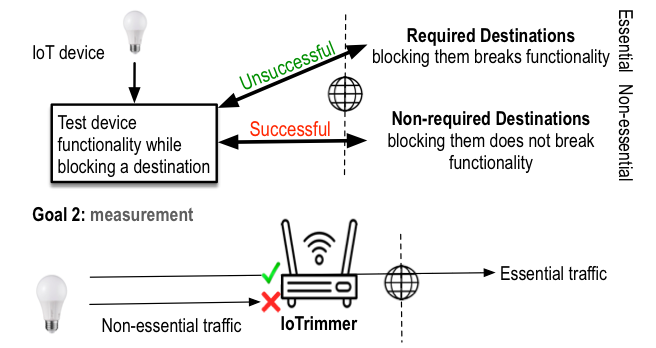
\includegraphics[scale=0.35]{main/countermeasures/pictures/IoTrimmer_IoTrigger}
    \caption{High-Level Architektur der Testumgebung für die Analyse des Netzwerkverkehrs der \ac{iot}-Geräte auf Basis von \textbf{Projekt 1} \cite{Mandalari2021}}
    \label{fig:test-setup-proj1}
\end{figure}

\noindent Die Identifikation der nicht essenziellen Endpunkte, die weder für die Bereitstellung der Service-Funktionalität des Gerätes verwendet werden noch für den Verwender von Nutzen sind, wurde auf Basis selbstentwickelter Werkzeuge in Form von Skripten, die auf den Routern der Testumgebung platziert wurden, durchgeführt. 
Eine genauere Betrachtung und Erläuterung der Funktionsweise dieser Werkzeuge folgt im späteren Verlauf dieser Ausarbeitung als Bestandteil der Sektion \fullref{sec:Regulationsmöglichkeiten} im Rahmen der Auswertung von Präventionsmöglichkeiten von nicht datenschutzkonformen Aktivitäten der Geräte im Smart Home.
Mittels dieses Experimentes konnte basierend auf den Funktionen der 31 getesteten Geräte eine Teilmenge von 16 Geräte identifiziert werden, die Daten an mindestens eine nicht benötigte Adresse zur Dienstbereitstellung senden. 
Die maximale Anzahl an blockbaren nicht benötigten Endpunkten lag im Kontext der ersten Untersuchung der Geräte bei elf Endpunkten. Diese Ergebnisse werden als Teil der nachfolgenden Grafik \ref{fig:result-non-req-dest} nochmals in Form eines Balken-Diagramms separiert der einzelnen Geräte-Typen dargestellt.

\begin{figure}
    \centering
    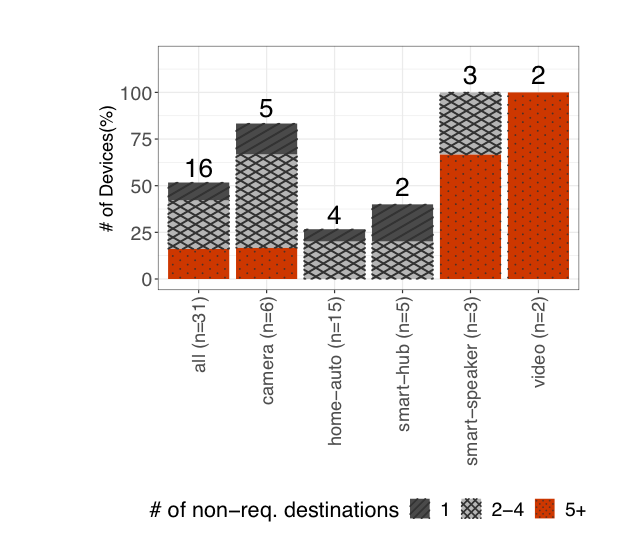
\includegraphics[scale=0.3]{main/pictures/projekt_one/Non_Required_Traffic}
    \caption{Ergebnisse der Analyse und Kategorisierung des Netzwerkverkehrs in essenziellen und nicht essenziellen Datenverkeht von \textbf{Projekt 1} auf Basis von \cite{Mandalari2021}}
    \label{fig:result-non-req-dest}
\end{figure}

\noindent Nach der Kategorisierung des gesammelten Netzwerkverkehrs wurde dieser anschließend nochmals in Kategorien bezüglich seiner finalen Ziele unterteilt. Die Unterscheidung wurde auf Basis von \textbf{First-Party}, \textbf{Support-Party} und \textbf{Third-Party} in Verbindung mit den aufgelösten Hostnamen vorgenommen, die nachfolgend nochmals genauer definiert werden.

\begin{itemize}
	\item \textbf{First-Party} sind Service-Endpunkte, die von den Geräteherstellern selbst bereitgestellt werden
	\item \textbf{Support-Party} beschreiben Endpunkte, die Support-Dienstleistungen für die einzelnen Geräte zur Verfügung stellen. Hierunter fallen beispielsweise Überwachung des Gerätestatus, Identifikation von Fehlfunktionen oder die Bereitstellung von Rechenkapazität für die Anwendungen.
	\item \textbf{Third-Party} Endpunkte sind wiederum Werbe- oder Marketing-Unternehmen, die die gesendeten Daten für marktanalytische Zwecke nutzen.
\end{itemize}

\noindent Resultierend aus dieser feingranulareren Unterteilung des Netzwerkverkehrs in die drei beschriebenen Kategorien, konnte die Erkenntnis gewonnen werden, dass beispielsweise der Datenverkehr an Endpunkte aus dem Bereich \textbf{Third-Party} nie für die Bereitstellung der Standardfunktionen eines \ac{iot}-Gerätes verwendet wird. 
Dieses Ergebnis wird nachfolgend nochmals in Form eines Balkendiagramms \ref{fig:result-non-req-dest-per-party} dargestellt, dass die Anzahl an Endpunkten gegen die fünf analysierten Geräte-Kategorien beschreibt. Hierbei kann in notwendige (rechts) und nicht notwendige Endpunkte (links) unterschieden werden. 

\begin{figure}
    \centering
    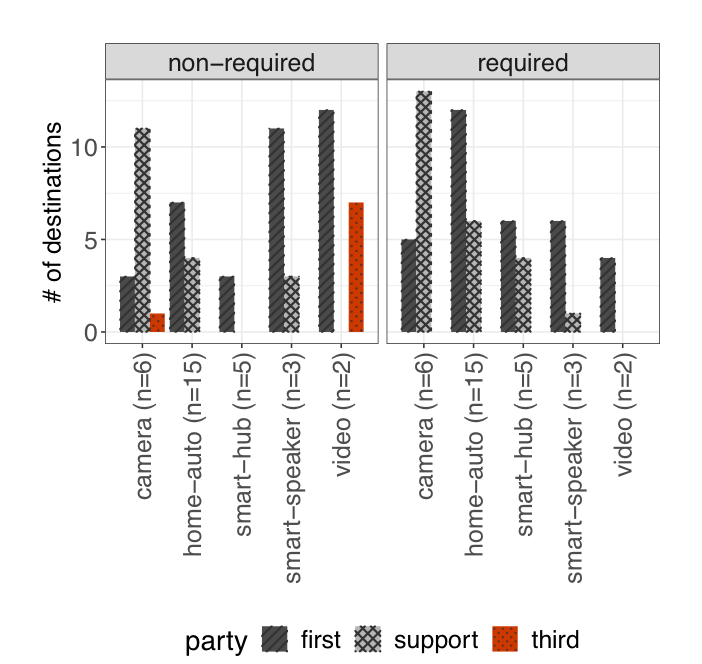
\includegraphics[scale=0.3]{main/pictures/projekt_one/Non_Required_Destination_Per_Party}
    \caption{Ergebnisse der Analyse auf Basis der feingranulareren Einteilung des Netzwerkverkehrs von \textbf{Projekt 1} auf Basis von \cite{Mandalari2021}}
    \label{fig:result-non-req-dest-per-party}
\end{figure}

\noindent Nach der Betrachtung der verwendeten Endpunkte innerhalb von \textbf{Projekt 1} wird der Versuchsaufbau von den 31 Geräten auf eine Grundgesamtheit von 81 Geräten in zwei unterschiedlichen Laboratorien in den USA und UK erweitert. 
Die zentrale Fragestellung beschäftigt sich hierbei mit der Auswirkung von unterschiedlichen Datenschutzregelungen auf das Verhalten der jeweiligen Geräte und die Art und der Umfang an Daten der durch die Dienstbereitstellung erhoben wird. Des Weiteren wird untersucht, ob sich aus den gesendeten Daten Implikationen auf die Privatsphäre des jeweiligen Nutzers ergeben.

\noindent Grundlegend ist der Versuchsaufbau derselbe geblieben und die Kategorisierung in die drei Endpunkt-Kategorien wurde aus dem vorherigen Projekt übernommen. Eine Erweiterung des Experimentes besteht in der Verknüpfung der beiden Testumgebungen durch einen VPN-Tunnel, um mögliches abweichendes Verhalten der Geräte in Abhängigkeit durch den Standort und somit auch die rechtlichen Regularien zu prüfen. 
Zudem wurde neben den bereits existierenden fünf Kategorien noch die Kategorie für \textbf{Heimgeräte} wie zum Beispiel Kühlschränke oder Waschmaschinen hinzugefügt, die eine Möglichkeit zur Steuerung über eine Nutzer-Schnittstelle auf dem Smartphone oder dem Web anbieten. 
Das Auslösen der einzelnen Aktivitäten, wie auch das Messen der Netzwerkaktivität der einzelnen Geräte im nicht benutzten Zustand ähnelt hierbei wieder dem ersten Projekt.

\noindent Auffälligkeiten bezüglich der Ergebnisse aus \textbf{Projekt 2} sind, dass von der allgemeinen Grundgesamtheit 72 Geräte mindestens einen Endpunkt mit Daten versorgen, der nicht zu dem eigentlichen Gerätehersteller gehört. 
Des Weiteren senden 56\% der Geräte in den USA und 83.3\% in den UK Endpunkte außerhalb ihrer Region. Dieses Verhalten wird nachfolgend durch \ref{fig:traffic-flow} mit der Illustration des ausgehenden Verkehrs von den einzelnen Gerätekategorien in deren Ziel-Länder nochmals übersichtlicher dargestellt. 

\begin{figure}
    \centering
    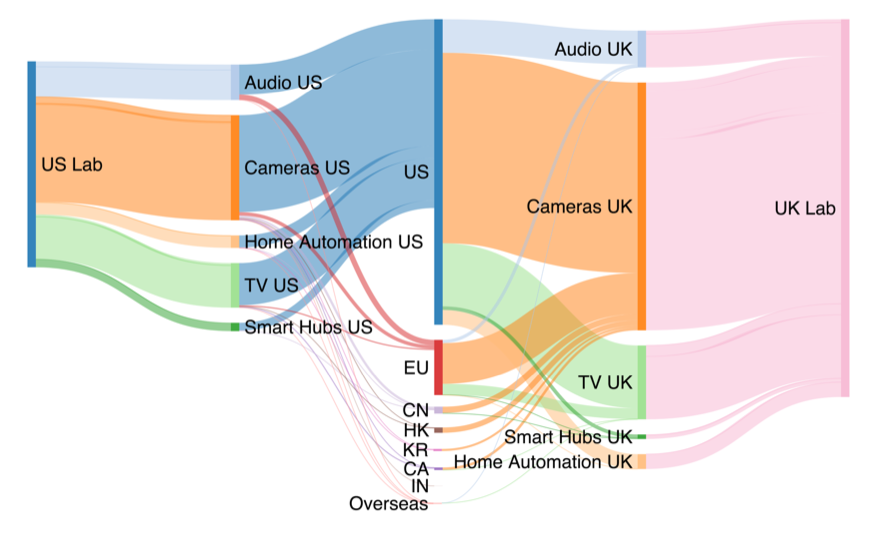
\includegraphics[scale=0.3]{main/pictures/projekt_two/Traffic_Flow_Destinations}
    \caption{Darstellung des Volumens an Netzwerkverkehr ausgehend von den einzelnen Geräten von \textbf{Projekt 2} \cite{Ren2019}}
    \label{fig:traffic-flow}
\end{figure}

\noindent Bezüglich dem Kontaktieren von \textbf{Support-} und \textbf{Third-Parties} wurde ein signifikanter Unterschied zwischen Geräten lokalisiert in den USA und in Europa identifiziert. 
In den meisten Fällen liegt hierbei die Rate von Geräten innerhalb der USA höher, wie im Vergleich zu ihren europäischen Gegenstücken. Eine genaue Auflistung der Menge an kontaktieren Endpunkten pro Gerätekategorie kann der nachfolgenden Tabelle \ref{table:non-first-party-by-device} entnommen werden. 
Die Deklarationen $US\cap$ $UK\cap$ beschreiben nur die Geräte, die in beiden Laboren vorkommen und die Deklaration $US \rightarrow UK$ und $UK \rightarrow US$ die Richtung des VPN-Tunnels aus dem jeweiligen Labor. 

\begin{table}
    \caption{Menge an Support- und Third-Parties kontaktiert bei den einzelnen Geräte-Kategorien aus \textbf{Projekt 2} \cite{Ren2019}}
    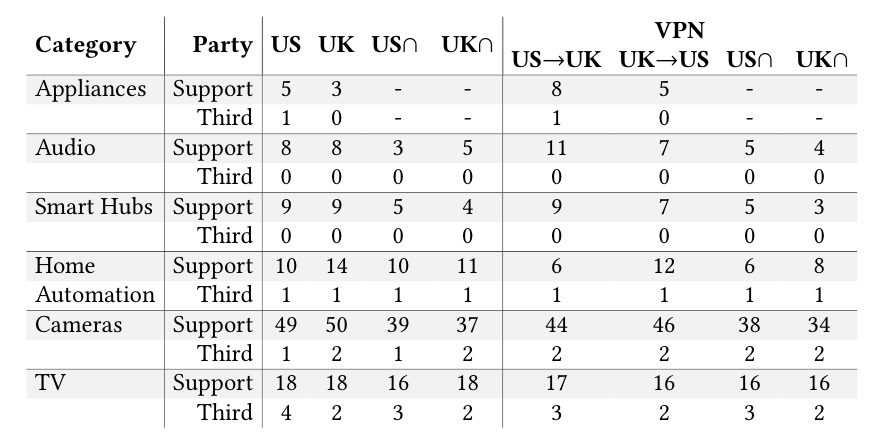
\includegraphics[width=\textwidth]{main/pictures/projekt_two/Non_First_Party_By_Category}
    \label{table:non-first-party-by-device}
\end{table}

\noindent Im Rahmen der Datenanalyse hinsichtlich dem Übertragen von \ac{pii} oder personenbezogenen Daten konnten nur wenige \ac{pii} innerhalb von unverschlüsseltem Netzwerkverkehr festgestellt werden. In vereinzelten Fällen tritt die Preisgabe von Geräte-ID, MAC-Adresse oder diversen UUIDs als unverschlüsselte Nachricht auf. 
Jedoch besteht bei 30 von 81 Geräten die Möglichkeit durch passives Mitschneiden von erzeugtem Datenfluss eine Rekonstruktion des Nutzerverhaltens, somit eine Kombination aus (User) Tracking und Profiling, durchzuführen. 
Zusätzlich konnte im Rahmen von unerwartetem Verhalten, das nicht von Nutzer initiiert wurde, bei drei Geräten ein Erhebung von Daten festgestellt werden, die nur teilweise dokumentiert und nicht durch eine Konfiguration des Gerätes durch den Nutzer deaktiviert werden kann. 
Hierbei handelt es sich nach der Definition der \ac{dsgvo} um personenbezogene Daten, die somit einen hohen Schutzstatus genießen. Die betreffenden Geräte und deren Geräte-Kategorie in Bezug auf deren Eigenheiten werden jedoch nicht als Teil dieser Arbeit genauer betrachtet und können in \cite{Ren2019} recherchiert werden.

%------------------------------------------------------------------------------------------------
\subsection{Smart City}
\label{sec:Analyse der Datenerhebung:ssec:Smart City}
%------------------------------------------------------------------------------------------------

Wie bereits in der Sektion \fullref{sec:Grundlagen} beschrieben, stellt die \textbf{Smart City} als übergeordneter Kontext den Zusammenschluss aus mehreren \textbf{Smart Environments} dar. Hingegen der Abgeschlossenheit einer \textbf{Smart Home} Umgebung ermöglicht sie, die Aggregation von Daten aus unterschiedlichen Bereichen des urbanen Lebens mit dem Ziel einer Verbesserung der Lebensqualität ihrer Einwohner. 
Die Konzepte dieses intelligenten Geflechts aus diversen Diensten in Kombination mit Sensoren beruhen somit auf einer besseren Interkonnektivität ihrer Teilkomponenten und einem daraus resultierenden erhöhtem Datenaustausch \cite{Stefanouli2019}. 
Diesbezüglich investieren weltweit Städte in den Ausbau und Einsatz von Technologien im Rahmen von Smart City Initiativen, um schwierige Aufgaben wie zum Beispiel die Nachhaltigkeit hinsichtlich der Umwelt, dem Verkehrsaufkommen innerhalb der Stadt, der Optimierung des öffentlichen Transports und der Gesundheit ihrer Einwohner zu adressieren \cite{BCG2020}.
Im Kontext der Kategorisierung der erhobenen Daten eine Analyse jeder Applikation oder eines jeden Systems innerhalb dieser einzelnen Ökosysteme vorzunehmen und hinsichtlich ihrer Datenschutzkonformität zu prüfen, ist jedoch nicht Teil der hier vorliegenden Arbeit und kann als Bestandteil zukünftiger Forschungsfragen zur Bewertung spezieller Teilbereiche einer \textbf{Smart City} definiert werden.
Um dennoch einen groben Überblick über die Applikationen innerhalb der einzelnen Querschnittsbereiche zu erlangen, werden diesbezüglich aus den bereits definierten fünf Bereichen einer Smart City jeweils ein Beispiel extrahiert und dieses anhand erhobener Daten analysiert und deren Funktionsweise vorgestellt.\\

%------------------------------------------------------------------------------------------------
\subsubsection{Smart Energy}
\label{sec:Analyse der Datenerhebung:ssec:Smart City:sssec:Smart Energy}
% Smart Energy: Smart Meter Beispiel
%------------------------------------------------------------------------------------------------

Bezüglich der Applikationen und Geräte des Teilbereichs \textbf{Smart Energy} findet das sogenannte \textbf{Smart Meter} innerhalb von \textbf{Smart Home} Instanzen häufigen Einsatz. Das Smart Meter beschreibt einen elektronischen Energiezähler, der in konfigurierbaren Intervallen automatisch den Energieverbrauch des jeweiligen Haushalts an den Energieversorger übermittelt. 
Weitere Funktionsmöglichkeiten sind die Auswertung der Daten beispielsweise über eine auf einem Computer im Heimnetzwerk installierte Software, um den persönlichen Stromverbrauch zu überwachen und in Kombination mit Solartechnologien einen Plan für die Verwendung von selbsterzeugtem Strom und dessen Rückeinspeisung in das Netz ermöglicht \cite{fox2010smart}. 
Die generierten Verbraucherprofile ermöglichen es den Netzbetreibern Lastprofile bezüglich ihrer Stromnetze zu erstellen und daraufhin durch Umleitungen aus weniger belasteten Bereichen des Netzes die Lastspitzen abzufangen. 
Somit findet eine Erhebung von Daten statt, die den Stromverbrauch eines Hauses in Bezug auf eine Geräte-ID widerspiegeln. Findet eine feingranularere Justierung der Zähler statt, sodass sie beispielsweise pro Stockwerk oder Zimmer den Verbrauch ermitteln können, lässt sich hiermit sogar die Verbindung zu einzelnen Personen herstellen.

%------------------------------------------------------------------------------------------------
\subsubsection{Smart Living}
\label{sec:Analyse der Datenerhebung:ssec:Smart City:sssec:Smart Living}
% Smart Living: Beispiel siehe Smart Home
%------------------------------------------------------------------------------------------------

Neben dem bereits beleuchteten \textbf{Smart Home} Kontext bietet \textbf{Smart Living} noch weitere Anwendungsbereiche wie beispielsweise \textbf{Social Network} oder die Umsetzung einer \textbf{Smart Community}. 
Da es sich bei der Smart Community eher um die Umsetzung eines Smart City Konzeptes handelt, werden die existierenden Applikationen des \textbf{Social Network} im Rahmen dieser Betrachtung herangezogen. Grundlegend steht im Kontext von Social Networking der Austausch von persönlichen Informationen auf virtuellen Plattformen, wie zum Beispiel Facebook oder Twitter, im Vordergrund. 
Durch die Verwendung dieser Apps soll es dem Nutzer ermöglicht werden persönlicher Inhalte aus dem seinem Privatleben oder Inhalte allgemeinen Interesses mit gleichgesinnten Nutzern in Form von Gruppen oder mit seinen direkten Kontakten zu teilen. Neben dem Verbreiten von Informationen werden diese Kommunikationskanäle auch zur Vernetzung mit Bekannten verwendet, die sich nicht im unmittelbaren Umfeld des Nutzers befinden. 
Aufnahmekriterium für jeden Nutzer der Plattform ist das Erstellen eines persönlichen Kontos oder Profils, auf dem er die Möglichkeit besitzt seine persönlichen Daten zu speichern und sich so für andere Nutzer identifizierbar zu machen. 
Abgesehen von den Ausnahmen von pseudonymisierten Profilen stellt der Großteil der Nutzer neben ihrem Namen und Geburtsdaten auch persönliche Interessen wie Hobbies auf ihre Nutzerprofile, die somit basierend auf ihren Privatsphäreeinstellungen, für den Rest der Plattform einsehbar sind. 
Dementsprechend befinden sich in diesem Teilbereich eine große Menge an personenbezogenen Daten im Umlauf, die von den Betreibern von sozialen Netzwerken erhoben und gespeichert werden.

%------------------------------------------------------------------------------------------------
\subsubsection{Smart Environment}
\label{sec:Analyse der Datenerhebung:ssec:Smart City:sssec:Smart Environment}
% Smart Environment: Beispiel für Wettersensoren
%------------------------------------------------------------------------------------------------

Die Domäne \textbf{Smart Environment} beschäftigt sich mit dem Zustand der Umwelt, in dem sich die \textbf{Smart City} befindet. Sie hat zum Ziel basierend auf Wetterdaten oder der Qualität der Luft ein vollumfängliches Lagebild der Stadt zu erstellen und durch Überwachungssysteme das Einhalten von Grenzwerten zum Beispiel bei der Kohlenstoffdioxid-Belastung zu garantieren. 
Weitere Anwendungsgebiete sind beispielsweise auch die Überwachung des Abwassers oder die Detektion von Waldbränden in der umliegenden Region \cite{SecPrivSmartCity2021}. Im Zusammenhang mit der Erfassung von Daten werden hier größtenteils nur technische beziehungsweise physikalische Informationen aus der Umwelt erhoben, die sich in Form von Temperatur oder Luftqualität wiederspiegeln. 
Eine direkte Verbindung zu einer Person kann hier nicht hergestellt werden. Eine andere Situation könnte sich ergeben, wenn beispielsweise Sensoren an jedem Abwasserkanal eines Hauses installiert und somit deren Abwasserproduktion überwacht werden würde. 
Dies käme einem Szenario ähnlich dem vorherigen Beispiel bezüglich des Einsatzes von \textbf{Smart Metern} innerhalb eines Haushaltes gleich. Hieraus erstellte Nutzerprofile könnten neben dem Verbrauch von Wasser zusätzlich die Zusammensetzung des Abwassers enthalten und mögliche Rückschlüsse auf die Verwendung bestimmter Produkte des Bewohners zulassen.

%------------------------------------------------------------------------------------------------
\subsubsection{Smart Industry}
\label{sec:Analyse der Datenerhebung:ssec:Smart City:sssec:Smart Industry}
% Smart Industry: Beispiel Kameras in den Fertigungshallen
%------------------------------------------------------------------------------------------------

Als kleinste Einheit wird im Kontext der \textbf{Smart Industry} die \textbf{Smart Factory} verstanden. Innerhalb dieser Fertigungsstätten arbeiten Menschen und Roboter Hand in Hand an der vollautomatisierten Herstellung eines Produktes. Die Besonderheit dieser Fabriken ist, dass sie aus mehreren sogenannten \ac{cpps} bestehen, die ausgestattet mit Prozessoren, Sensoren und Servomotoren physikalische Prozesse innerhalb der Anlage steuern \cite{Sadeghi2015}. Für die Gewährleistung eines reibungslosen Produktionsablaufes erheben die \ac{cpps} Daten der einzelnen bearbeiteten Produkte und ihrer unmittelbaren Umgebung und tauschen diese im Verbund untereinander aus. Dies ermöglicht es beispielsweise, dass jedes \ac{cpps} zu genau jedem Zeitpunkt Kenntnis davon hat, wo sich das zu bearbeitende Produkt innerhalb der Fabrik genau befindet und welcher Arbeitsschritt gerade durchgeführt wird. Neben den reinen produktspezifischen Daten interagieren die \ac{cpps} auch mit menschlichen Nutzern und sammeln somit durch Aufnahmen mit visuellen oder Sprachsensoren auch Daten der Mitarbeiter, die an den entsprechenden Maschinen tätig sind.

%------------------------------------------------------------------------------------------------
\subsubsection{Smart Services}
\label{sec:Analyse der Datenerhebung:ssec:Smart City:sssec:Smart Services}
% Smart Services: Erläuterung der BCG Analyse der Parkplatz-Reservierungs-App
%------------------------------------------------------------------------------------------------

Die Bereitstellung von Diensten aus dem Bereich \textbf{Smart Services} umfasst neben intelligenten Lösungen für die Handhabung des Verkehrs innerhalb einer \textbf{Smart City} wie in \ref{sec:Grundlagen} beschrieben zusätzlich Lösungen bezüglich der öffentlichen Verwaltung, dem Gesundheitswesen und dem Transport \cite{SecPrivSmartCity2021}. Bei genauerer Beachtung der Servicedienstleistungen lässt sich abstrahieren, dass in jedem dieser Kontexte die Interaktion mit einem Bewohner einer \textbf{Smart Citiy} inbegriffen sein muss.
Bedeutet, die Handhabung und Verarbeitung personenbezogener Daten ist eine notwendige Bedingung, um die jeweilige Funktion hinreichend anzubieten. Beispielsweise wäre die Verwendung einer Applikation für das Finden eines Parkplatzes nicht unbedingt zielführend, wenn sie keinen Zugriff auf den Standort des Nutzers und seiner umliegenden Umgebung hätte. 
Wiederum hieraus lässt sich schließen, dass diese Art von Anwendungen nicht nur aus einzelnen Datentöpfen bedient werden können, sondern einen Querschnitt an Informationen über unterschiedliche Bereiche hinweg erfordert. 
Diese Problematik des Datenaustausches innerhalb von Smart City Applikationen wurde bereits in \cite{BCG2020} schwerpunktmäßig analysiert. Ziel der Auswertung war es, ob Smart City Anwendungen für die Bereitstellung ihrer Dienste, wie zum Beispiel einer Parkplatz-Reservierungs-App, nur Informationen aus einer Quelle beziehen oder einen Längsschnitt durch andere Bereiche ziehen. 
Bereiche wurden in diesem Kontext als Industriezweige definiert, die somit eine besondere Verantwortung für die von ihnen erhobenen Daten besitzen. Bezüglich der angesprochenen Parkplatz-Reservierungs-App konnte festgestellt werden, dass neben den Belegungsdaten von Garagen, historischen Verkehrsdaten und aktuellen Wetterdaten auch Informationen über baldige öffentliche Veranstaltungen verwendet werden, um in Echtzeit die Parkkosten für bestimmte Bereiche innerhalb der Stadt zu prognostizieren. 
Dieses Ergebnis lies sich im Rahmen der angestellten Untersuchungen von 75 Applikationen in diesem Umfeld mindestens die Hälfte Daten über mehrere Quellen hinweg aggregiert und für die Dienstbereitstellung verwendet. 
Darunter waren Anwendungen des öffentlichen Transports und der Verwaltung am Häufigsten vertreten. Veranschaulicht wird dies als Teil des nachfolgenden Diagramms \ref{fig:data-aggregation-smart-city-apps}, das neben den aktuell existierenden Anwendungen zusätzlich noch mögliche zukünftige Projekte umfasst, von denen bereichsübergreifend Daten gesammelt werden.

\begin{figure}
    \centering
    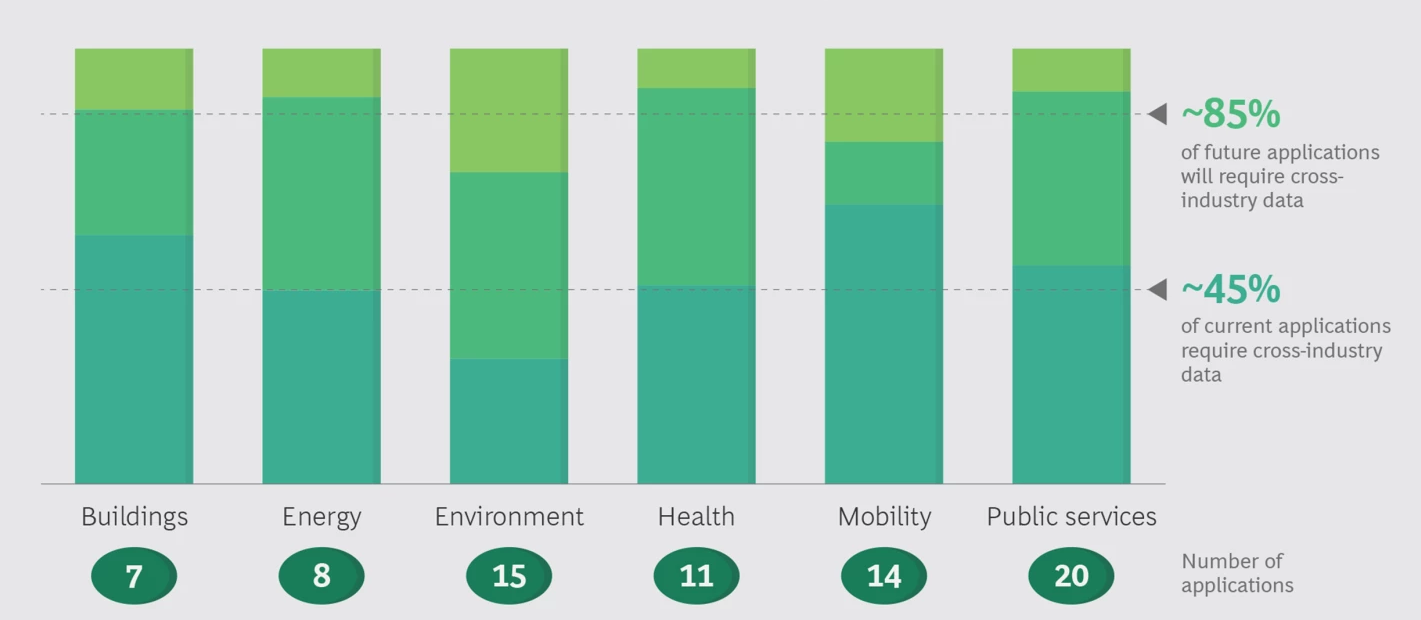
\includegraphics[scale=0.2]{main/pictures/smart_city/Smart_City_Apps_Data_Req}
    \caption{Übersicht über die Menge an Applikationen, die Daten über mehrere Industriezweige zur Service-Bereitstellung aggregieren \cite{BCG2020}}
    \label{fig:data-aggregation-smart-city-apps}
\end{figure}

\noindent Im Hinblick auf die erhobenen Daten können bei der beispielhaft betrachteten Applikation durchaus personenbezogene Daten identifiziert werden. Daraus resultiert, dass der vorgefundene Datenaustausch über mehrere Grenzen smarter Umgebungen hinweg, nicht ohne Nutzung von Regularien zur Handhabung dieser Daten rechtmäßig stattfinden darf.\\

%------------------------------------------------------------------------------------------------
\subsection{Bewertung der Datenschutzkonformität}
\label{sec:Analyse der Datenerhebung:ssec:Bewertung der Datenschutzkonformität}
%------------------------------------------------------------------------------------------------
% Smart Home Bewertung
Basierend auf der umfassenden Betrachtung von beispielhaften Applikationen aus dem Bereich \textbf{Smart Home} und der übergeordneten Domäne \textbf{Smart City} wird anschließend anhand der identifizierten erhobenen Informationen nun die Datenschutzkonformität kontextübergreifend bewertet. 
Im Rahmen dieser Bewertung werden jedoch keine genaueren Betrachtungen hinsichtlich der einzelnen Anwendungen und Systeme selbst angestellt, sondern nur auf dessen aktuellen Zustand hin die Beachtung der derzeit geltenden Rechtssprechung im Rahmen der \ac{dsgvo} und dessen Einhaltung festgestellt.
Beginnend mit den Anwendungen und Geräten des \textbf{Smart Home}, die im Rahmen der beiden Arbeiten \cite{Mandalari2021,Ren2019} auf deren Verhalten und die Preisgabe von personenbezogenen Daten untersucht wurden, konnte festgestellt werden, dass einzelne Geräte zu der Zeit der Analyse nur bedingt \ac{dsgvo}-konformes Verhalten aufwiesen. 
In Anbetracht der beiden Grundprinzipien der \ac{dsgvo} hinsichtlich \textbf{Datenminimierung} und \textbf{Zweckbindung} wurden während der Nutzungsphasen und Ruhephasen der Geräte dennoch Daten erhoben, die beispielsweise bei der betrachteten intelligenten Türklingel Bildmaterial mit zugehörigem Zeitstempel enthielten, ohne dass der Nutzer Einfluss auf den Prozess der Datenerhebung genommen, beziehungsweise diese Aktion gewünscht ausgelöst hat. 
Zwar bestünde hier die Möglichkeit der Argumentation für den Hersteller im Rahmen einer besseren Dienstbereitstellung zusätzliche Daten zu erheben, um den Service zu optimieren \cite{Bastos2019}. Jedoch würde dies hingegen der Verbesserung des Service-Angebots der Einwilligung des Nutzers bedürfen, die in dem obigen Beispiel von Seiten der Dienstbetreiber und Gerätehersteller nicht eingefordert wurden. 
Ferner ist neben der Prüfung zweckmäßiger und angemessener Datenerhebung das Versenden an entsprechende Endpunkte zur Dienstbereitstellung ein zentraler Punkt der zweiten Studie. Im Rahmen der \ac{dsgvo} wird hierbei von der Verarbeitung oder Speicherung in sogenannten "Drittländern" \cite{dsgvo2016} gesprochen, die wiederum in sichere und unsichere Länder unterteilt werden können. 
Wie aus der Darstellung \ref{fig:traffic-flow} zu entnehmen ist, werden Informationen aus dem Labor in Großbritannien an Destinationen gesendet, die sich beispielsweise in den USA (\textbf{US}) und in China (\textbf{CN}) befinden. Diese sind im Rahmen der Drittländer-Regelung nicht ohne weiteres als sichere Verarbeitungsländer geführt und bedürfen somit gesonderten Regelungen für die rechtmäßige Übertragung. 
Bezüglich der Datenübermittelungen in die USA ist dies auf die für ungültig erklärte Privacy Shield Reglung \cite{dsgvo2016} zurückzuführen, womit Daten nur unter Anfertigung erweiterter Schutzrichtlinien an amerikanische Dienste gesendet werden dürfen. Ob diese Abkommen für die einzelnen Geräte im Kontext ihrer Nutzung angefertigt und eingehalten werden, lässt sich jedoch ohne eine genauere juristische Prüfung nicht bestimmen und war auch nicht Teil der Studien. 
Einzig die Ergebnisse aus der Untersuchung der verschlüsselten und nicht verschlüsselten übertragenen Informationen waren im Rahmen der \ac{dsgvo} bis auf wenige Ausnahmen konform gegenüber den Regularien \cite{Ren2019}. Nur in wenigen Fällen konnten \ac{pii} in Form von Geräte-ID oder IP-Adressen als personenbezogenes Datum identifiziert werde.
Bedeutet, dass speziell für \textbf{Smart Home} auf Basis der Ergebnisse aus dem erhobenen Zeitraum für einige Geräte ein Potential für Optimierung besteht, um die Einhaltung der derzeit geltenden Rechtssprechung im europäischen Raum zu gewährleisten.
Im Zuge der im letzten Jahr eingeführten Standards \textbf{ETSI EN 303 645} \cite{Cyber2020} besteht nun neben der Option der Bewertung der erhobenen Daten zusätzlich eine Möglichkeit zur Prüfung der Konzeption bezüglich Sicherheit in Bezug auf die Architektur der erstellten Systeme speziell für den Smart Home Kontext. Da es jedoch bei der vorliegenden Arbeit hauptsächlich um den Datenschutz dieser Systeme geht, kann diese Referenz als Formulierung zukünftiger Schwerpunkte für Analysen herangezogen werden.\\
% Smart City Bewertung
Im nächsten Schritt erfolgt Einstufung der Anwendungen und Systeme aus dem Kontext der \textbf{Smart City}. Aufgrund des größeren Betrachtungswinkels werden die erläuterten einzelnen smarten Umgebungen in ihrer Gesamtheit als \textbf{Smart City} bewertet. Basierend auf den unterschiedlichen Bereichen, wie bereits in der Sektion \ref{sec:Analyse der Datenerhebung:ssec:Smart City} erläutert, lässt sich die Datenerhebung und Verwendung meist nicht auf nur einzelne Teilbereiche und ihre Domänen eingrenzen und erfordern somit diesen notwendigen Grad an Abstraktion.
Wie aus der Analyse \cite{BCG2020} ersichtlich, findet zur Service-Erbringung in den meisten Fällen eine Aggregation an Daten statt, die aus mehreren Quellen gezogen werden. Hierbei besteht jedoch die Gefahr, dass bei Erheben von personenbezogenen Daten, wie zum Beispiel dem personenbezogenen Datum des Standorts einer Person mit ihrem Fahrzeug bei Parkplatz-Apps, besondere Sicherheitsvorkehrungen für die Bearbeitung eingehalten werden müssen.
Wird der Fokus von Applikationen, die sich in der Regel auf den Smartphones der jeweiligen Benutzer befinden und somit in der Regel generell häufiger mit personenbezogenen Daten in Kontakt kommen, wie beispielsweise smarte Komponenten einer Infrastruktur, bestehen auch beispielsweise bei \ac{tms} Risiken hinsichtlich der Erhebung von Daten einzelner Verkehrsteilnehmer.
Als Beispiel lässt sich zur Erläuterung der Problematik das Projekt "SmartWalk" \cite{SmartWalk2022} in Hamburg heranziehen, das unter Verwendung von Kamera-Systemen die sichere Überquerung von Fußgängern an besonders befahrenen Straßen regeln soll. 
Hierzu werden von den Sensoren und Kameras Bilddaten der einzelnen Fahrzeuge und Fußgänger erfasst, die als Datengrundlage für explizite Entscheidungen für das Regeln des Verkehrs herangezogen werden. Im Rahmen der \ac{dsgvo} handelt es sich somit um \textbf{biometrische} und \textbf{Standortdaten}, infolgedessen personenbezogene Daten. 
Bedeutet, die Verarbeitung und das Teilen mit anderen Anbietern von Diensten aus demselben Bereich ist somit nicht ohne weiteres möglich. Herangehensweisen, die dennoch eine sichere Verarbeitung dieser Daten außerhalb des Gerätes ermöglichen wird als Teil der nachfolgenden Sektion \ref{sec:Regulationsmöglichkeiten} genauer betrachtet. 
Entsprechend der Einhaltung der Konformität bezüglich der \ac{dsgvo} lässt dies jedoch den Schluss zu, dass ohne eingebaute Vorkehrungen innerhalb der Systeme oder Anwendungen zur Präprozessierung der Daten oder Prinzipien wie \ac{sbd} und \ac{pbd} keine Herstellung eines unbedenklichen Datenschutz-Status herbeigeführt werden kann. 
Diese Problematik lässt sich aufgrund des in den meisten Anwendungen verwendeten Datenaustausches über mehrere Industriezweige hinweg \cite{BCG2020} als Abhängigkeit in andere Kontexte der Smart City übertragen.
In Anbetracht der bereits gescheiterten Projekte wie das Smart City Projekt von Google Sidewalks Lab in Toronto \cite{SidewalkToronto2022} konnte stets das Fehlen der Optionen zur Regulation der Erhebung und dem Austausch der von den Einwohnern erhobenen Daten, als einer der Hauptgründe für den Misserfolg der jeweiligen Unternehmung identifiziert werden \cite{Bernier2022}.
Ähnliche Arbeiten, die bezüglich des Big Data-Begriffs die Anwendung von Applikationen und Systeme der \textbf{Smart City} innerhalb der europäischen und amerikanischen Rechtssprechung analysierten, kamen bezüglich der unterschiedlichen Rechtssprechungen zu ähnlichen Ergebnissen.
Resultierend wurde festgestellt, "dass Big-Data-Anwendungen [Applikationen einer Smart City], welche sich [...] in der Smart City realisieren lassen, mit den in unserem Rechtskreis geltenden datenschutzrechtlichen Grundsätzen in einem prinzipiellen Spannungsverhältnis stehen. Lässt sich dieses nicht auflösen, können die betreffenden Geschäftsmodelle nicht rechtmäßig umgesetzt werden" \cite[p.~45]{Sennhauser2019}. 
Nach der ernüchternden Bewertung der beiden smarten Kontexte werden nachfolgend Möglichkeiten zur Regulation der Systeme aufgezeigt, die es den Nutzern oder auch den Herstellern der Anwendungen während des Betriebs oder bereits in der Entwicklung auf die Einhaltung der \ac{dsgvo} zu achten und das unerwünschte Erheben personenbezogener Daten zu präventieren.
